\documentclass{article}

\usepackage[utf8]{inputenc}
%\usepackage[english]{babel}
\usepackage[T1]{fontenc}
\usepackage{microtype}

\usepackage{newspaper}

\date{\today}
\currentvolume{1}
\currentissue{2}

%% [LianTze] The newspaper package also provides 
%% these commands to set various metadata:

%% The banner headline on the first page
%%   (The colon after s: is to get a more
%%   modern majuscule s in this font instead of 
%%   the medieval tall s. For anyone interested 
%%   in the history: 
%%  http://medievalwriting.50megs.com/scripts/letters/historys.htm)
\SetPaperName{XignalX, Inc. Press}

%% The name used in the running header after
%% the first page
\SetHeaderName{XignalX, Inc. Press}

%% and also...
\SetPaperLocation{Delaware, USA}
\SetPaperSlogan{\textit{Who is going to believe a con artist? Everyone, if she is good.}}
\SetPaperPrice{\$ 1.05}


% [LianTze] times (the package not the font) is rather outdated now; use newtx (see later)
% \usepackage{times}

\usepackage{graphicx}
\usepackage{multicol}

\usepackage{picinpar}
%uasage of picinpar:
%\begin{window}[1,l,\includegraphics{},caption]xxxxx\end{window}
\newcommand{\NewsAuthor}[1]{
		    \textsc{#1} \vspace{4pt}
			\par \normalfont}	

%% [LianTze] Contains some modifications
\usepackage{newspaper-mod}
%%... so now you can redefine the headline and byline style if you want to.
%% These can be issued just before any
%% byline or headline in the paper, to
%% individually style each article
%%
% \renewcommand{\headlinestyle}{\itshape\Large\lsstyle}
% \renewcommand{\bylinestyle}{\bfseries\Large\raggedright}


%%%%%%%%%  Front matter   %%%%%%%%%%

\usepackage{lipsum}

\begin{document}
\maketitle

\begin{multicols}{2}

\byline{Con Men, Conspiracy and Nazis}{Matthew Woods}

\begin{window}[2, c, 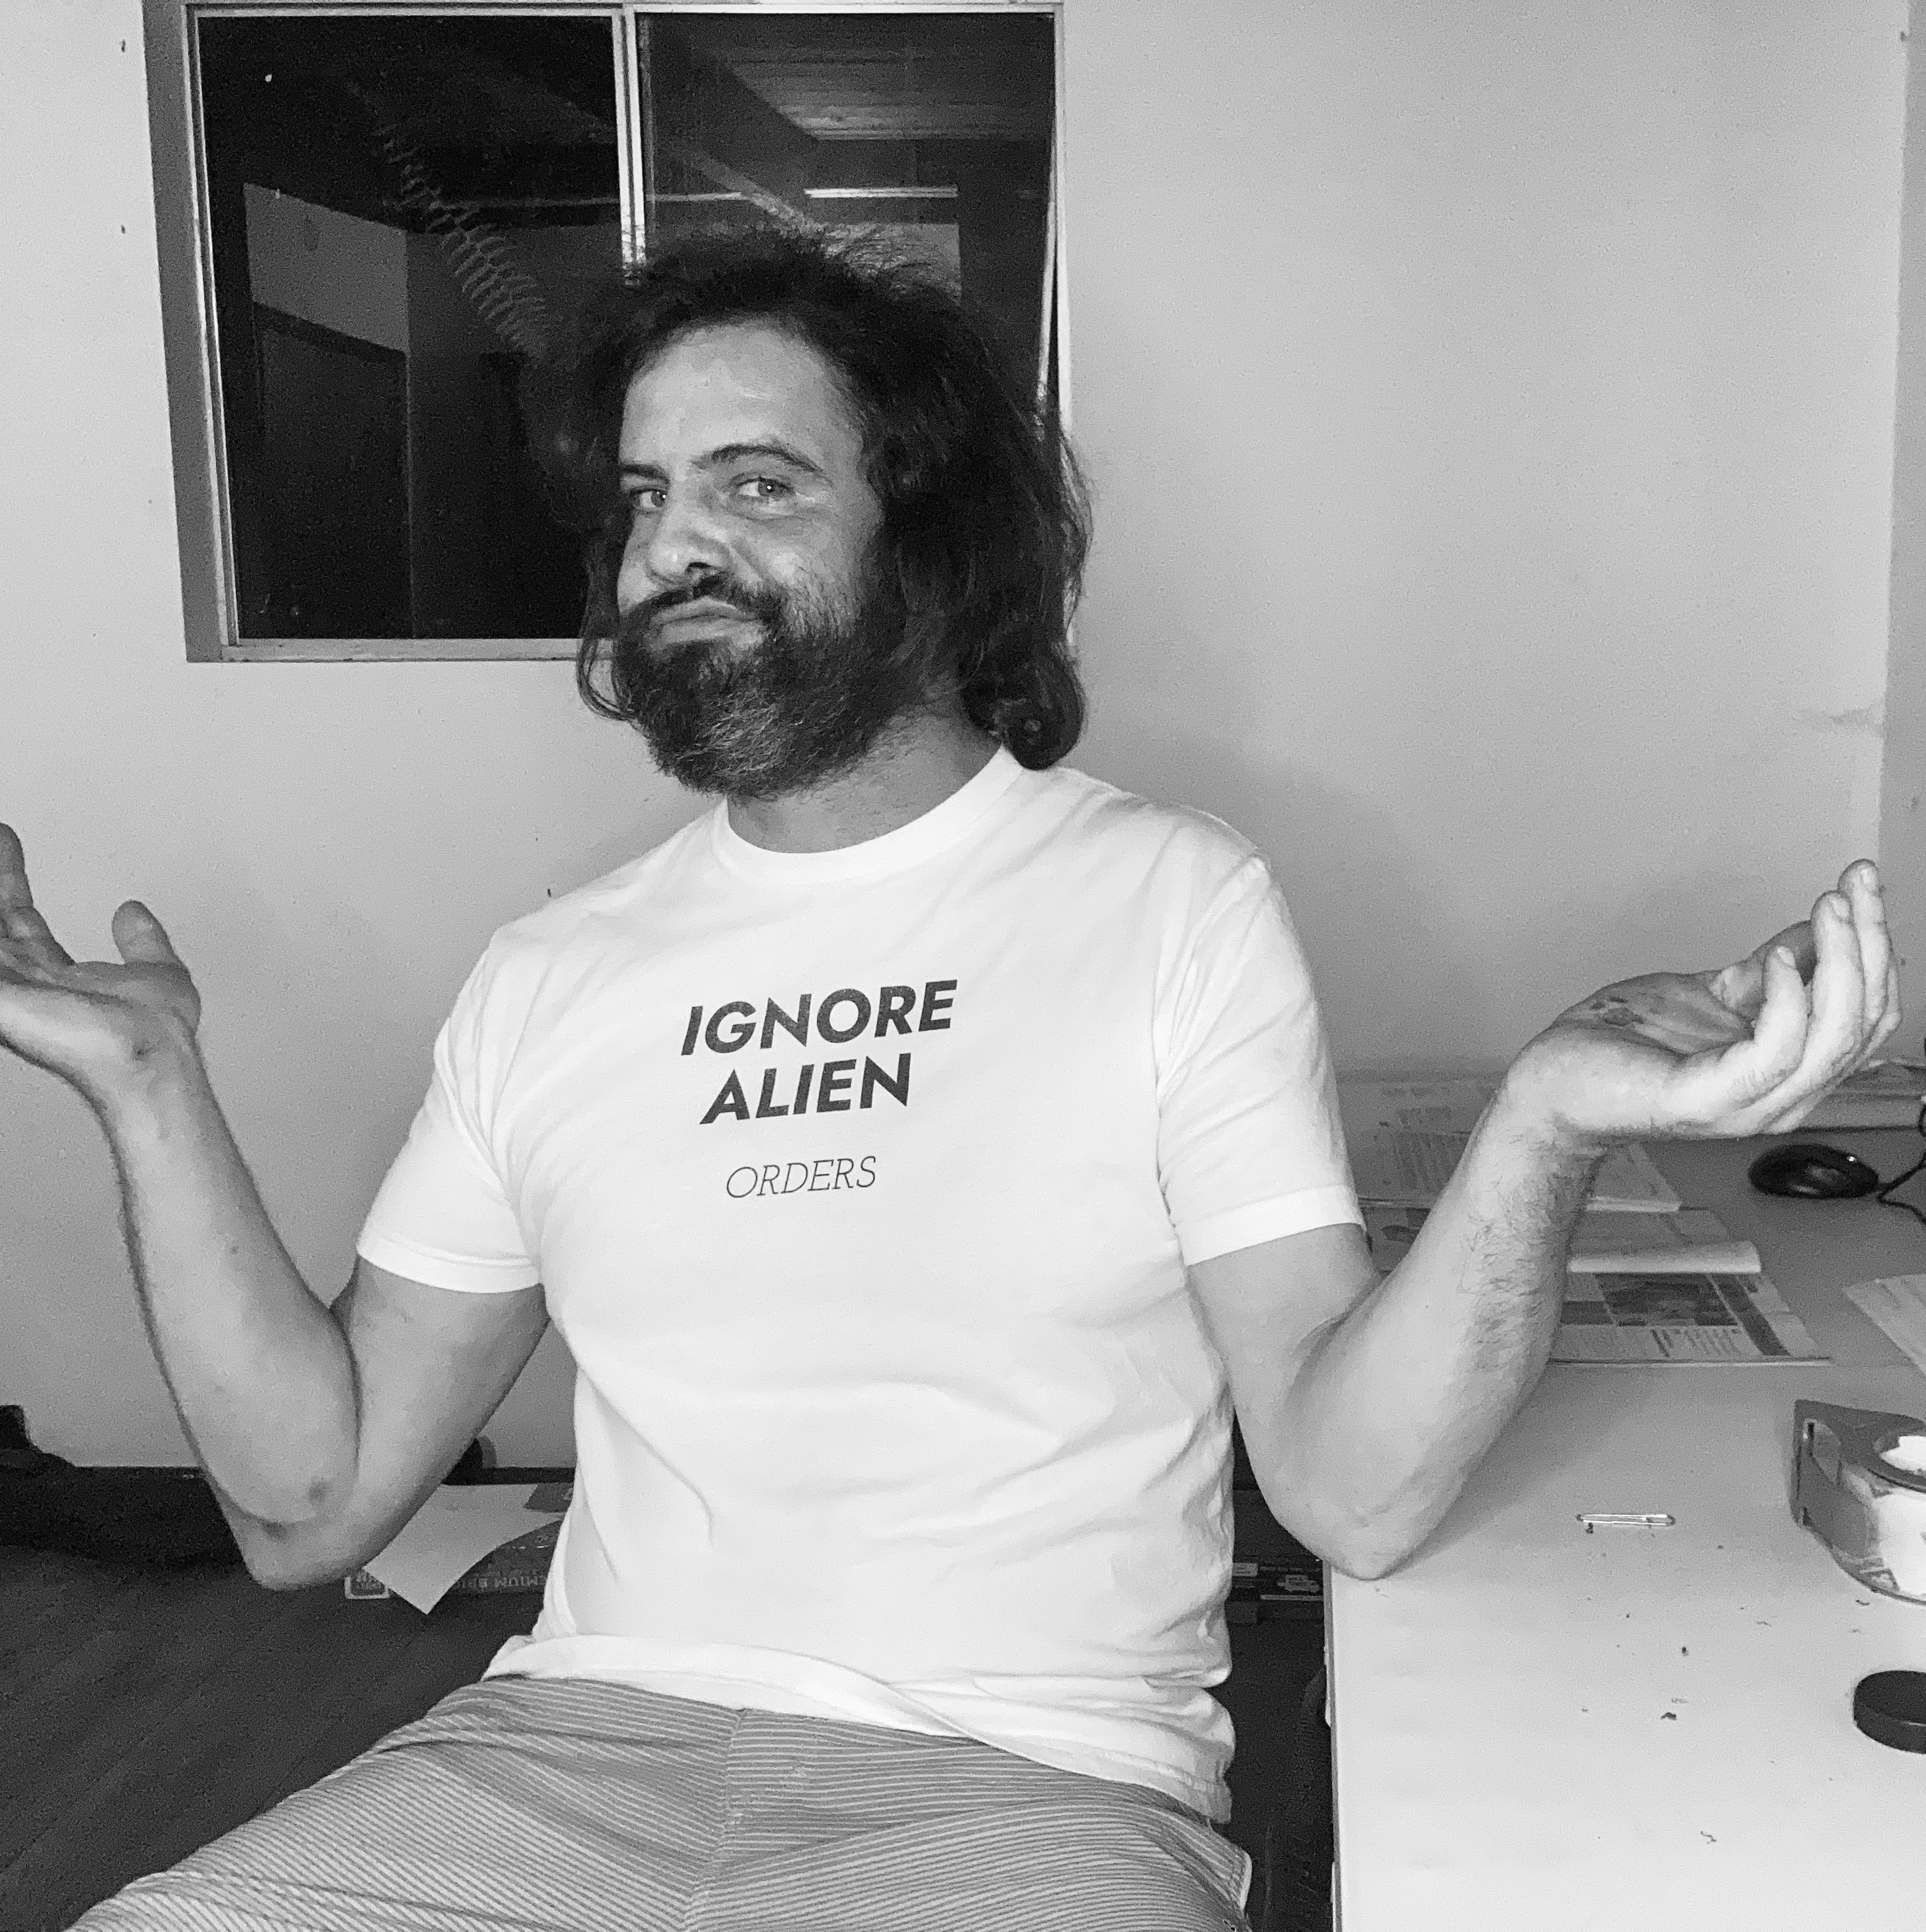
\includegraphics[width=2.8in]{profilepic.jpeg},\centerline{\textit{mattwoods243@outlook.com}}] 
\end{window}

Between the years of 2015 and present, I have been the victim of multiple con conspiracies; it was so vast that I could not even believe it myself at first. I thought that I had gone insane. In retrospect, it appears that they were “Crazy Making” me with large numbers of people. The scope of the con included family, friends, coworkers, professionals, police, hotels, hospitals and more. I was 14 years old and living in Pennsylvania the first time something like this happened to me. I never understood then, yet I moved on and never experienced anything similar until 2015. My consensus is that my family played a role in all of these cons. They are Nazis: psychopaths who organize conspiracies around me without me knowing it. I can’t imagine to what end, since they started with me so early. Perhaps making a weak useful idiot that they could control was the goal. Thankfully I never listened to them: they failed. When I was 18 I joined the Navy and never looked back, certain that whatever nonsense I had been experiencing with them would cease. I could not have been more wrong.

Rise up warriors. Take your stand at one anothers sides. Set our feets wide and rooted like the oak in the ground. Learn to love death's inky black shadow as much as you love the light of dawn. Here is courage:  masnkind's finest possesion and the  noblest prize that a young man can posses: courage, in the unlikely event, and so forth. 

\end{multicols}

\closearticle

\end{document}
